% !TeX root = ../main.tex
% Add the above to each chapter to make compiling the PDF easier in some editors.
\chapter{Design and Implementation}\label{chapter:design}

\section{Technology Stack}
In order to implement the architecture proposed in Chapter \ref{chapter:method} we choose Android as end user device platform. Android has the highest market share among mobile devices \cite{android-market-share} and offers a healthy ecosystem of frameworks and libraries that simplify development. Furthermore we opted for an implementation in Kotlin instead of Java to reduce boilerplate code and improve readability.

As server side technology we choose node.js in conjunction with a mongoDB object store database. A NoSQL database like mongoDB provides flexibility and easy adaption of data schemes without much overhead and thus perfectly fits our prototyping purpose. We choose node.js out of the same reasons. In contrast to a statically typed language, javascript provides more flexibility and ease of change. Furthermore, node.js is often used in combination with mongoDB and provides seamingless integration.

The aggregation results are made available to the public via a dedicated route of the server but might also be made available directly through granting access to the respective collection\footnote{A collection in an object store is the equivalent to a table in an SQL database.} of the database.

The following sections describe the implementation of the Android application as well as the server and explain design decisions. We start with an outline of the API shared by both, the Android application and the server.\\

\section{API}\label{api}
%shared by the Server and the Android Application
\subsection{Overall API Architecture}
The API is designed as a REST API based on JSON data exchange format and consists of the endpoints listed in Table \ref{api-endpoints}.

\begin{table}[h]
  \begin{tabularx}{\textwidth}{|l|X|}
    \hline
    \multicolumn{2}{|c|}{\textbf{Data Consumption from 30.05.2019 - 04.06.2019}}                                                                              \\ \hline
     \multicolumn{1}{|c|}{\textbf{HTTP call}}                 & \multicolumn{1}{c|}{\textbf{Description}}                                                                               \\ \hline
    POST /user HTTP/1.1                & Creates a new user and corresponding password (see Fig.\ref{post-user-request} and \ref{post-user-response}) \\ \hline
    POST /forward HTTP/1.1             & Sends a processed aggregation request back to the server (see Fig.\ref{post-request})              \\ \hline
    POST /admin/sampleRequest HTTP/1.1 & Saves and initiates a new aggregation (see Fig.\ref{insert-sample})                                          \\ \hline
    GET /requests?pk=... HTTP/1.1      & Retrieves aggregation requests for a user (see Fig.\ref{get-requests-response})                    \\ \hline
    GET /aggregations HTTP/1.1         & Retrieves all aggregation results (see Fig.\ref{get-aggregations})                                 \\ \hline
  \end{tabularx}
  \caption{Description and usage of API endpoints shared by the Android application and the server.}
  \label{api-endpoints}
\end{table}

\begin{figure}[!h]
  \begin{lstlisting}[language=json,firstnumber=1]
  {
    "publicKey": "-----BEGIN PUBLIC KEY-----\nMIIBIjANBgkqhkiG..."
  }
  \end{lstlisting}
  \caption{Body of an HTTP request for creating a new user.}
  \label{post-user-request}
\end{figure}

\begin{figure}[h!]
  \begin{lstlisting}[language=json,firstnumber=1]
  {
    "publicKey": "-----BEGIN PUBLIC KEY-----\nMIIBIjANBgkqhkiG...",
    "password": "LSFDfzduSFSozfwf"
  }
  \end{lstlisting}
  \caption{Body of an HTTP response upon successful creation of a new user.}
  \label{post-user-response}
\end{figure}

\begin{figure}[h!]
  \begin{lstlisting}[language=json,firstnumber=1]
  [{
    "publicKey": "-----BEGIN PUBLIC KEY-----\nMIIBIjANBgkqhkiG...",
    "serverId": "acfbdxxfceoelaOdkfeecIf",
    "nextuser" : "-----BEGIN PUBLIC KEY-----\nMIIBIjANBgkqhBms...",
    "encryptionKey":"HXporXstqrgkfsCpezlqZcpLb...",
    "iv":"pMxQznHqbzeZuzVLfiFHYQ==",
    "encryptedRequest":"xtgPteNAeAKEhfPXQeZt..."
  }]
  \end{lstlisting}
  \caption{Body of an HTTP response listing all aggregation requests for the specified user.}
  \label{get-requests-response}
\end{figure}

\begin{figure}[h!]
  \begin{lstlisting}[language=json,firstnumber=1]
  {
    "publicKey": "-----BEGIN PUBLIC KEY-----\nMIIBIjANBgkqhkiG...",
    "password": "LSFDfzduSFSozfwf",
    "serverId": "acfbdxxfceoelaOdkfeecIf",
    "encryptionKey":"HXporXstqrgkfsCpezlqZcpLb...",
    "iv":"pMxQznHqbzeZuzVLfiFHYQ==",
    "encryptedRequest":"xtgPteNAeAKEhfPXQeZt..."
  }
  \end{lstlisting}
  \caption{Body of an HTTP request sending the processed aggregation request back to the server.}
  \label{post-request}
\end{figure}

\begin{figure}[h!]
  \begin{lstlisting}[language=json,firstnumber=1]
  [{
    "timestamp": 1559216514521,
    "startedAt": 1559216514685,
    "start": "2019-05-28",
    "end": "2019-05-31",
    "type": "steps",
    "n": 6,
    "value": 4271,
    "valueList": []
  },
  {
    "timestamp": 1559216514521,
    "startedAt": 1559216514685,
    "start": "2019-05-28",
    "end": "2019-05-31",
    "type": "stepsListing",
    "n": 5,
    "value": 0,
    "valueList": [1661, 1246, 3195, 7714, 7842]
   }]
  \end{lstlisting}
  \caption{Body of an HTTP response listing all completed aggregations.}
  \label{get-aggregations}
\end{figure}

\begin{figure}[h!]
  \begin{lstlisting}[language=json,firstnumber=1]
  {
    "password": "adminPassword",
    "start": "2019-05-31",
    "end": "2019-06-05",
    "type": "activity_2",
  }
  \end{lstlisting}
  \caption{Body of an HTTP request for initiating a new aggregation.}
  \label{insert-sample}
\end{figure}

The routes used for interaction with the application (except the one for creating a new user) are secured and can only be accessed if the user can be authenticated successfully. The routes for initiating new aggregations and retrieving all results require administrator authentication (see Fig. \ref{insert-sample}). We used Postman [TODO: Link] to initiate aggregations. The collections [ref!!!] are here. The route for the results is designed to be available to the public without authentication. Nevertheless we restrict access in this test setup to fully protect users' privacy.\\
On creation of a new user, the server response contains a password randomly generated for the user to be used for authentication in all future server communication as e.g. in Fig. \ref{post-request}. All aggregations waiting to be processed by the user and also the respective responses (see Fig. \ref{post-request} and \ref{get-requests-response}) contain the public key of the user to identify which user should handle the request. Furthermore, the request contains a field \textit{encryptionKey} which is a synchronous key, encrypted with the user's public key. This synchronous key in combination with the initialization vector \textit{iv} has been used to encrypt the actual aggregation request described in Chapter \ref{chapter:method} and send along in it's encrypted version in \textit{encryptedRequest}. The \textit{serverId} is the identifier of the request used by the server's database.
%So, for example, our experimental trajectory request type is not available to the public.

%The encryptedRequest field e.g. in figure \ref{get-requests-response} contains the encrypted version of the request .

%//TODO: Integrate this section somewhere else (in methodology)
\subsection{Data Aggregation Design}\label{data-aggregation-design}
All aggregations proposed in section \ref{aggregation-schemes} can be implemented using only 4 fields: An Integer \textit{n} specifying the current number of participants, a Floating Point Number \textit{value} containing e.g. the current mean value of the aggregation, a list \textit{valueList} of Floating Point Numbers that can be reused for different purposes accross requests and a String \textit{type} that specifies the request type. The request type specifies the used scheme, i.e. how the other fields are populated e.g. the encoding of the \textit{valueList}. In addition, all aggregation requests have a start day and an end day. Days' time is always treated as 00:00 o'clock. Thus, the timespan for an aggregation is always a multiple of 24 hours. Fig. \ref{get-aggregations} shows two examples of completed aggregations which highlight the reusability of the 4 fields. They furthermore contain a \textit{timestamp} when the aggregation has been completed and when it had been started (\textit{startedAt}).\\

\begin{samepage}
Due to limited scope of this thesis, only the following out of the aggregation requests defined in section \ref{aggregation-schemes} were implemented:
\begin{enumerate}
	\item Computing the average number of steps walked across all users participating in the aggregation.
	\item Computing the average time spent walking, running, in a vehicle or on a bicycle \parencite{detected-activity}.
	\item Collecting a list of the average number of steps walked by each participant during the timespan.
\end{enumerate}

In addition, we implemented another aggregation in order to test our setup and the data quality:
\begin{enumerate}
  \setcounter{enumi}{3}
  \item Collecting a list of all trajectories registered by the users' phones.
\end{enumerate}
\end{samepage}

The implementation of additional aggregations is straight forward and requires only few changes and additions using the provided setup. All aggregations work as a prove of concept of the proposed setup and hence serve answering research question 1. Aggregation 1, 2 and 3 furthermore help to investigate which types of aggregations are possible to be published and allow for an investigation whether overlapping timeperiods allow for inference attacks. Thus, they help to answer research question 2 and 3. Especially aggregation 3 in comparison with aggregation 1 and 2 allow for answering research question 2.
Aggregation 4 imposes a privacy risk on the user as discussed in \parencite{twitter, cellphone, krumm} and was only implemented in order to get an overview of the data quality of our setup and validate the feasability of the other aggregation requests proposed in section \ref{aggregation-schemes}.

\section{Android Application}\label{android-app}
The Android application targets Android Oreo (API level 27) and requires a minimum API level of 19. Approximately 96.8\% of devices run on this or a higher version of Android \cite{android-api-level-share} which allows our application to be installed on the majority of Android devices.
Furthermore, the application leverages Goolge Play Services to obtain GPS and activity data. Without Google Play Services installed, the application will not work. In order to ease future adaptability, we chose to use the Dagger2 framework \parencite{dagger} for dependency injection in order to decouple classes as far as possible. Further use of frameworks and libraries will be explained in the following respective sections.

\begin{samepage}
The application is aimed at collecting GPS data, detecting the user's current activity and counting the user's steps. The data collection process happens in the background without any user interaction required. Aggregation requests to aggregate data accross devices are also served without the need of any user interaction.
The Android application can be grouped into three main parts of loosely coupled modules:
\begin{itemize}
	\item A module responsible for collecting and saving raw data.
	\item A module responsible for locally aggregating raw data.
	\item A module responsible for communicating with the server and handling aggregation requests.
\end{itemize}
\end{samepage}

\begin{figure}[h!]
  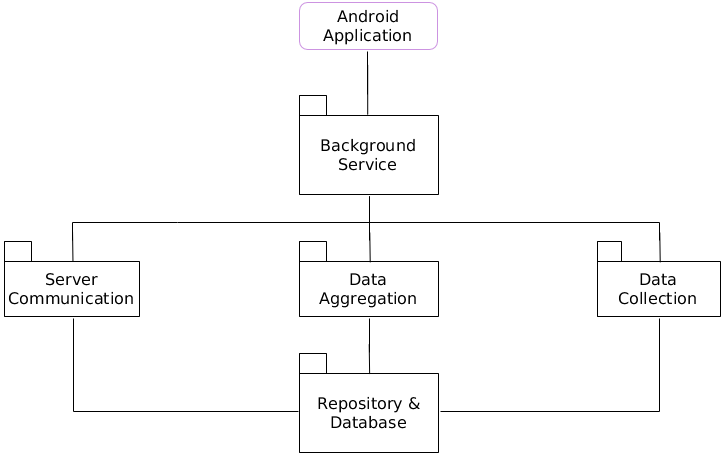
\includegraphics[width=\textwidth]{data/diagrams/android-architecture.png}
  \caption{Layered Android architecture with three decoupled main modules controlled by the background service.}
  \label{android-overview}
\end{figure}

The control flow as depicted in Fig. \ref{android-overview} is as follows: 
The Android application has only one Main Activity in order to ask the user to allow location access and start the background service. Apart from that, this Activity does not serve any specific purpose. 
The data collection, the local aggregation and the polling of new requests from the server happen in the background on a 15 minute interval and are initiated by the background service. The Android Workmanager then controls this periodic work without any user interaction being required.

For the App in order to have maximum possibilities collecting especially GPS data and preventing the Android operating system from entering doze mode when not interacted with by the user, a non-dismissible status notification is displayed at all time\footnote{Compare to the non-dismissible status notification displayed by Google Maps when the navigation system is active.}. Also, the application is registered to be automatically restarted upon boot\footnote{From Android 6.0 on (API level 23), apps' behaviour is restriceted by the operating system in order to reduce battery consumption. E.g. all apps are automatically managed by the battery manager which restricts background launches \parencite{background, doze}. The user has to switch this option to manual management in order to allow the app to be started in the backgorund after boot.} and also when the application is closed by the user (e.g. via the task manager) so that once installed, no further user interaction is necessary.
Furthermore, the application, respectively each module is heavily unit tested in order to guarantee functionality and facilitate further development by other research teams. Unit and integration tests are based on AndroidJUnit4 \parencite{androidJunit4} and the espresso \parencite{espresso} framework.


\subsection {Data Collection}
We choose to separate the aggregation and collection of location data in order to decouple the modules and provide the possibility to extend the model of aggregated data in the future without the need to change the raw data model. Vice versa the data collection process can be modified without impacting the aggregation process.\\

We use the Android Room Persistence library \parencite{room} to store data locally. The library provides a layer over the standard SQLite database commonly used by many Android applications. We collect three types of data:
\begin{itemize}
	\item Steps: If available, the phone's internal step sensor provides updates on a regular basis. The step sensor always informs about the total number of steps since the last reboot. Upon each time we receive data from the step sensor, this data is stored directly in the \textit{step\_counter\_table}.
	\item User's activities: The Google Play Services  activity recognition API leverages different data and sensors available on the phone in order to inform about the most probable current activity of the user as one of \textit{still, walking, running, in a vehicle, on bicycle} \parencite{detected-activity}. Whenever there is a change detected, two events are fired - one for exiting the previous and one for entering the current activity. The events might not be dispatched instantly but contain the timestamp of the exact occurence. Upon each received event, this data is stored directly in the \textit{activity\_transition\_table}.
	\item GPS positions: GPS data is retrieved through the \textit{FusedLocationProviderClient} which leverages cellphone-tower and WIFI data apart from GPS to determine the position. In order to limit battery consumption, GPS data is only requested every minute if the device's detected activity is \textit{still}\footnote{Neertheless, if other applications request a GPS position, our application also receives this data, even if it occurs on a faster interval.}. If the current detected activity is \textit{walking}, the interval is set to 5 seconds and in any other state, the interval is set to every second. The data is stored in the linked tables \textit{gps\_data\_table} and \textit{gps\_location\_table}. We choosse to separate the GPS point itself from the timestamp having in mind that future aggregations might need or leverage the separation of spatial data and time and more than one event might be attached to the same GPS point.
\end{itemize}

\subsection{Local Data Aggregation}\label{local-data-aggregation}

\begin{table}[]
  \centering
  \begin{tabular}{|l|l|l|l|}
    \hline
    \multicolumn{4}{|c|}{\textbf{Sample GPS data set}}           \\ \hline
    \textbf{Id} & \textbf{Latitude} & \textbf{Longitude} & \textbf{Timestamp} \\ \hline
    1 & 44              & 11         & 10:11:03    \\ \hline
    2 & 44.5            & 11.1       & 10:11:15    \\ \hline
    3 & 44.4            & 11.05      & 10:12:12    \\ \hline
    4 & 44.3            & 11.07      & 10:33:00    \\ \hline
    5 & 44              & 11.2       & 10:34:00    \\ \hline
    6 & 44.00001        & 11.2       & 10:36:10    \\ \hline
    7 & 44              & 11.2       & 10:38:23    \\ \hline
  \end{tabular}
    \caption{Sample GPS data input for calculating trajectories.}
  \label{algo-input}
\end{table}

From the received values of the step counter since last reboot saved in \textit{step\_counter\_table} the number of daily steps is computed and stored in \textit{steps\_table}. The exit and enter events received via the activity recognition framework and stored in the \textit{activity\_transition\_table} are matched in order to compute activities with start and duration properties. Those activities are then saved in the \textit{activity\_table}.
GPS data is used to compute trajectories through the following algorithm examplarily applied to the sample GPS data in Table \ref{algo-input}:
\begin{enumerate}
	\item When there are more than 10 minutes between two subsequent GPS points in the sequence of all GPS points to be processed, the sequence is separated into two separate sequences and each is processed separately as a possible trajectory in the next step. Regarding the sample data, the GPS points with the ids 1, 2 and the GPS points with the ids 3, 4, 5 would be treated as separate sequence.
	\item Furthermore, we identify still moments - periods of no movement - as follows:
	\begin{enumerate}
		\item For each GPS point, we identify a subsequent GPS point that was registered at least two minutes after the first one. For example, regarding the GPS point with id 1, the GPS point with id 4 is the first one with at least two minutes in between.
		\item If the average speed between those two points calculated from the time and the distance between the points is below 0.6 m/s, the pair is added to a list to be processed in the next step. This is the case e.g. for the pairs with the ids 5, 6 as well as the pair of 6, 7.
		\item The list of pairs of GPS points resulting from the last step is fused into sequences of GPS points as long as possible: Whenever two pairs overlap in their timespan, they are fused to a new pair covering the combined timespan and consisting of the first pair's first GPS point and the last pair's last GPS point. An example here is the sequence from id 5 to 7.
	\end{enumerate}
	\item The GPS pairs of still moments resulting from the last step are used to exclude still moments from the original sequence of GPS points and hence divide it into subsequences each defining a single trajectory. In the example the resulting sequences are 1,2,3 and 4,5.
\end{enumerate}
Of each trajectory, the start and end location as well as the respective timestamps are then saved in the \textit{trajectory\_table}. We tested 0.5 m/s, 0.6 m/s and 0.7 m/s as threshold in step 2b and found 0.6 m/s to fit the tested sample the best. On the one hand, the threshold must be low enough to still include slow walking which might be below 1 m/s. On the other hand, the threshold should not be too low because inaccuracy in GPS data might otherwise induce trajectories where the device has actually not moved at all.

\subsection{Serving Aggregation Requests}
We use the retrofit2 framework \parencite{retrofit} based on OkHttp \parencite{okhttp} to handle communication with our REST server described in Section \ref{server}. An HTTP Interceptor is used to modify incoming and outgoing requests. The interceptor decrypts the request body of incoming messages using the private key of the installation before the body is parsed into Java Objects. On outgoing messages, the interceptor adds authentication before sending them to the server.
The app polls for new aggregation requests every 15 minutes. New aggregation requests are first stored locally in the database. Those requests are then processed and the results are again stored locally as pending outgoing requests until they are finally send to the server. This separation of concerns is useful especially in case of an interrupted communication during processing the aggregation request. When the results cannnot be send to the server, the app automatically retries the next time that the communication module is invoked.\\
The aggregation process itself takes the \textit{type} parameter of the request to specify which actions to take on the three fields (\textit{n:Int, value:Float, valueList: List<Float>}) shared across all aggregation requests. In case of the types \textit{steps} and \textit{activity\_X} the field \textit{value} contains the current mean of the data and the field \textit{n} is the number of participants so far. In case of \textit{stepsListing} only the field \textit{valueList} is used. Each user's mean value is added to the list. In case of \textit{trajectories}, only the field \textit{valueList} is used; four subsequent elements of the list always represent one trajectory as of latitude of start position, longitude of start position, latitude of end position and longitude of end position.

In case that the aggregation should be changed to actually work over P2P, e.g. using local WIFI networks, only the communication module has to be adapted to the new routing of requests. No further changes to the application are necessary.

\section{Server Design and Implementation}\label{server}
The server is build using the event-driven node.js verion 10.15.3 leveraging the express web-server framework \parencite{express} and using the mocha testing framework \parencite{mocha} in combination with the chai assertion library \parencite{chai} for unit and integration testing. The server is designed using a layered architecture as described in Fig. \ref{server-architecture}. On the lowest level are the data models which define and verify the data schemes defined in subsection \ref{server-data-model}. The \textit{commonRepository} and the \textit{userRepository} are build on top of these models and persists data in a mongoDB object store. They also handle transactions where several objects are modified subsequently. The third level provides the logic to be executed for each endpoint defined in \textit{routes.js}. On the top level, \textit{server.js} starts the server on the specified port, registers the routes described in Section \ref{api}, respectively adds authentication and interacts directly with the \textit{userRepository} in order to update the respective users \textit{lastSeen} property. Furthermore, it starts a scheduled repeating task in order to bypass users in the aggregation chain that have not responded to their aggregation request after a certain time. This process is described in Section \ref{request-chain}.

\begin{figure}[h!]
  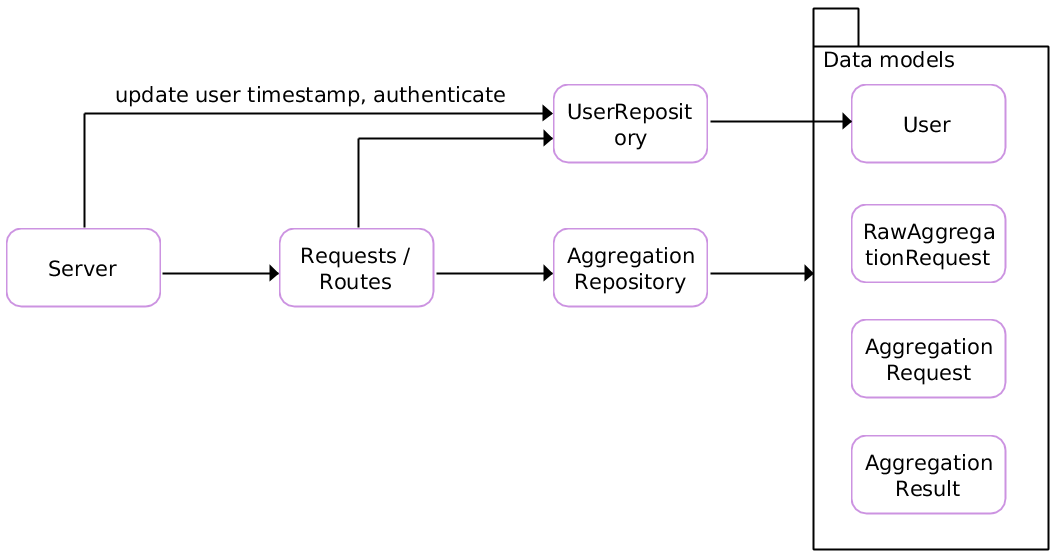
\includegraphics[width=\textwidth]{data/diagrams/server-diagram.png}
  \caption{Layered Server architecture with repositories and data models on a separate layer.}
  \label{server-architecture}
\end{figure}

\subsection{Data Model}\label{server-data-model}
We organize the data in four collections. The user collection stores the user data which is the corresponding public key, the hashed password and \textit{lastSeen} - the timestamp of the last interaction of the user with the server. Aggregation requests are split into two collections. The collection \textit{rawAggregationRequests} stores the initial aggregation request inserted through the admin interface containing the fields start, end, and type. Furthermore, the three fields n, value, valueList reused across all aggregations, the timestamp when the request was filed to the server and a flag indicating whether this request has already been started \footnote{In case of a newly inserted aggregation where the end date is in the future, the request will be started only when this day has passed.} are stored. Upon start of an aggregation request, a list of the 10 most recently active users is retrieved in order to serve this request. The request body is then encrypted with the first user's public key and stored in the collection \textit{aggregationRequests"}. Each time, a user requests an \textit{aggregationRequest}, proceeds with it and sends the result back to the server, the result is inserted into the database as a new \textit{aggregationRequest}. The fields of this collection are described in Table \ref{aggregationRequest}.

\begin{table}[]
  \centering
  \begin{tabularx}{\textwidth}{|l|X|}
    \hline
    \multicolumn{2}{|c|}{\textbf{Fields of \textit{aggregationRequest}}}                     \\ \hline
     \multicolumn{1}{|c|}{\textbf{Name}}        & \multicolumn{1}{c|}{\textbf{Purpose}}       \\ \hline
    rawRequestId     & The id of the related \textit{rawAggregationRequest} . This field is not available through the API. \\ \hline
    started\_at      & The timestamp, when the request was started. \\ \hline
    publicKey        & The public key of the next user that should process this request.   \\ \hline
    nextUser        & The public key of the user that will receive the request afterwards. This is necessary so that the user that should process this request can encrypt the processed request with the public key of the next user.
     \\ \hline
    previousRequest        & The id of the previous request which is null, if it is the first request in the chain. This field is used by the process described in Section \ref{request-chain} in order to bypass a not responding user in the chain.
     \\ \hline
    users        & A list of public keys of the following users that will proceed with this request. This field is not available through the API.
     \\ \hline
    encryptionKey        & A synchronous key used to encrypt the request itself. The synchronous key in turn is encrypted with the public key of the user the request is aimed at.
     \\ \hline
    iv        & The initialization vector used for synchronous encryption and decryption of the actual aggregation request.
     \\ \hline
    encryptedRequest        & The actual aggregation request encrypted with the synchronous key. \\ \hline
    timestamp        & The timestamp when this object has been created. \\ \hline
    completed        & A flag indicating whether this aggregation request has already been processed by the respective user.
     \\ \hline
  \end{tabularx}
    \caption{Fields of the collection \textit{aggregationRequest}.}
  \label{aggregationRequest}
\end{table}

\begin{samepage}
The last collection called \textit{aggregationResults} is used to store the results of an aggregation request. Once there are no more users to serve an aggregationRequest, the last user sends the final data unencrypted to the server where it is stored as an \textit{aggregationResult}. It contains the same fields as the \textit{rawAggregationRequest} except the \textit{started} flag. Additionally, it contains the fields \textit{started\_at} and \textit{timestamp} - indicating when the aggregation request referenced through \textit{rawRequestId} was started and when it was completed.
\end{samepage}

\subsection{request-chain}\label{request-chain}
//TODO
server.js also invokes a scheduled task which re-routes stale requests where the user has not proceeded with the pending request either due to being offline or due to a problem handling the request. When new aggregation requests are started, the lastSeen timestamp of users is taken into account to exclude users that have not connected for a certain time. Furthermore, the list of users who are selected to serve the new request is ordered by the time the user was last seen.